\documentclass[tikz,border=10pt]{standalone}
\usepackage[T1]{fontenc}
\usepackage{tgheros}
\usepackage{sfmath}
\usepackage{amsmath}
\usepackage{tikz}
\usetikzlibrary{arrows.meta,positioning,shapes.geometric,fit,backgrounds,calc}
\usepackage{xcolor}

\renewcommand{\familydefault}{\sfdefault}

% Academic Semantic Palette (Harvard Crimson & ETH Zurich)
\definecolor{ethdarkblue}{HTML}{1F407A}
\definecolor{ethblue}{HTML}{215CAF}
\definecolor{ethbronze}{HTML}{B87333}
\definecolor{harvardcrimson}{HTML}{A51C30}
\definecolor{ethpurple}{HTML}{5B4B8A}
\definecolor{ethpetrol}{HTML}{007A87}
\definecolor{ethslate}{HTML}{334155}
\definecolor{cardbg}{HTML}{F8FAFC}
\definecolor{cardborder}{HTML}{CBD5E1}
\definecolor{subtlebg}{HTML}{F1F5F9}

\begin{document}
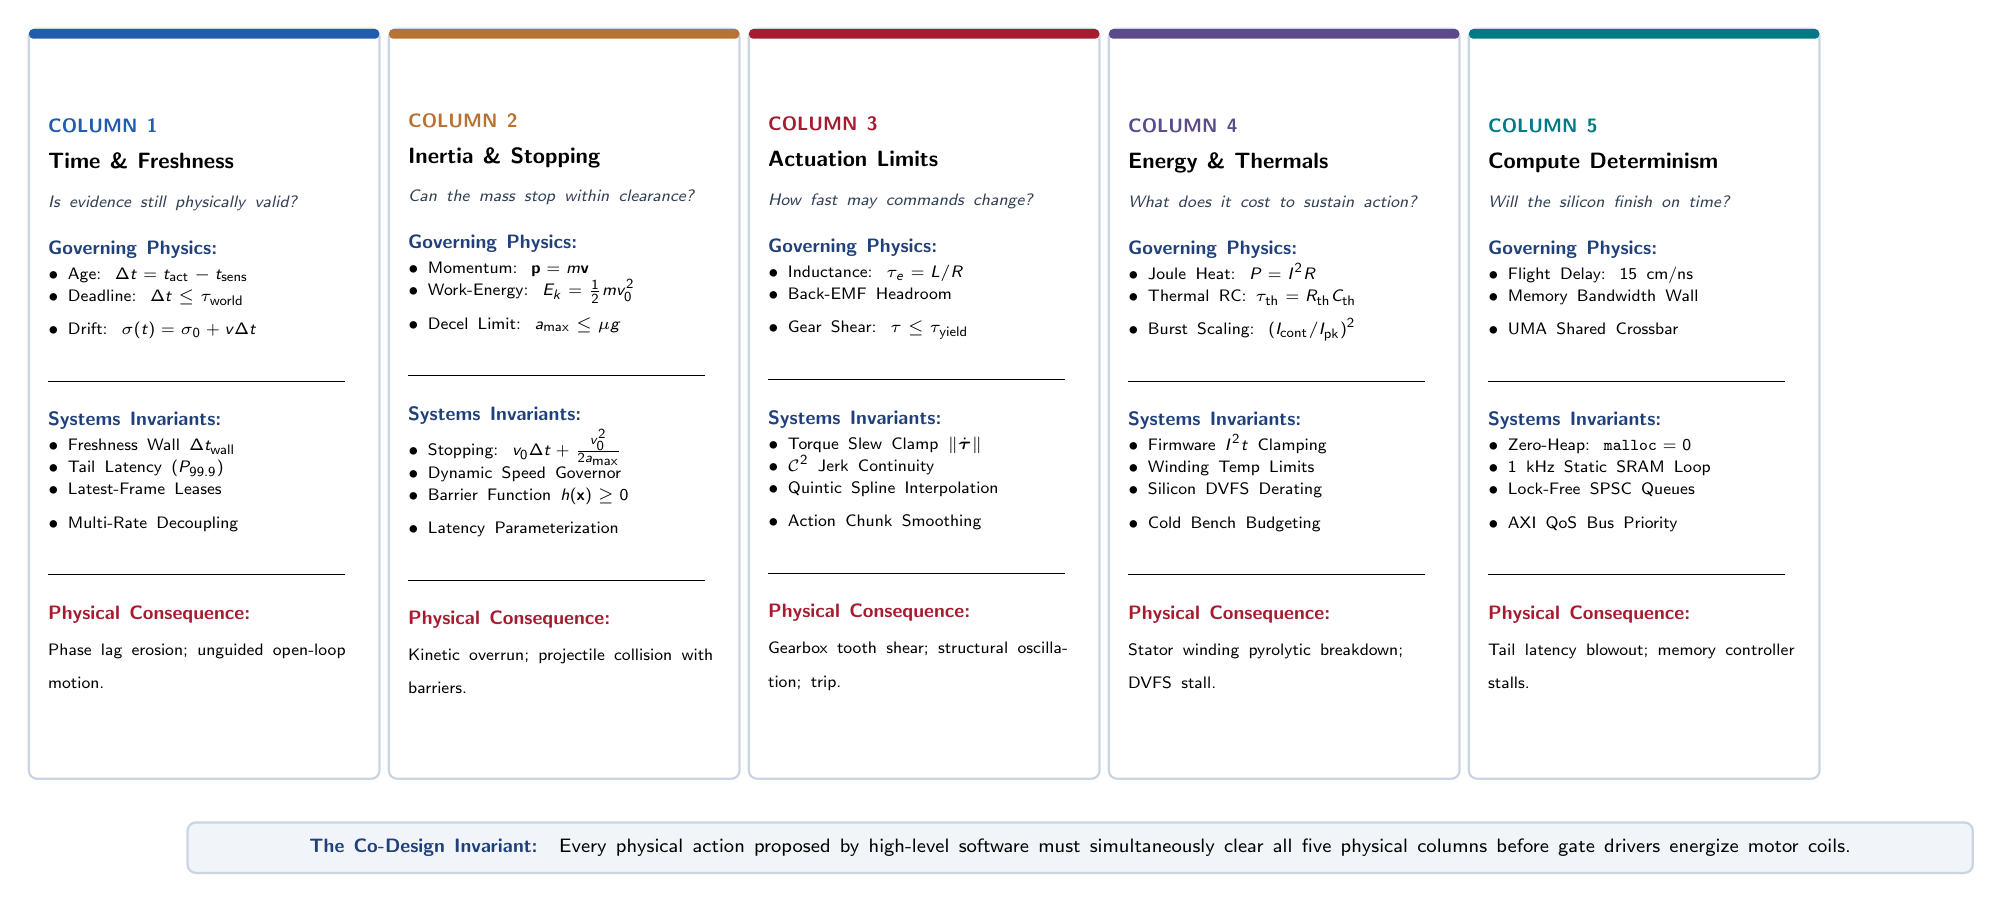
\begin{tikzpicture}[
  font=\sffamily,
  >=Stealth,
  scale=1.0,
  columncard/.style={
    draw=cardborder,
    fill=white,
    rounded corners=3pt,
    line width=0.8pt,
    text width=1.56in,
    minimum height=3.75in,
    inner sep=7pt,
    align=left,
    anchor=north
  }
]

  % ---------------------------------------------------------------------------
  % COLUMN 1: Time & Information Freshness
  % ---------------------------------------------------------------------------
  \node[columncard] (col1) at (0, 0) {
    {\fontsize{7pt}{8.5pt}\selectfont\bfseries\color{ethblue}COLUMN 1}\\[1pt]
    {\fontsize{8.5pt}{10.5pt}\selectfont\bfseries Time \& Freshness}\\[2pt]
    {\fontsize{6.5pt}{8pt}\selectfont\itshape\color{ethslate}Is evidence still physically valid?}\\[5pt]
    
    {\fontsize{7pt}{8.5pt}\selectfont\bfseries\color{ethdarkblue}Governing Physics:}\\[1pt]
    {\fontsize{6.5pt}{8pt}\selectfont
    $\bullet$ Age: $\Delta t = t_{\text{act}} - t_{\text{sens}}$\\
    $\bullet$ Deadline: $\Delta t \le \tau_{\text{world}}$\\
    $\bullet$ Drift: $\sigma(t) = \sigma_0 + v\Delta t$}\\[5pt]
    
    \rule{0.95\linewidth}{0.3pt}\\[4pt]
    {\fontsize{7pt}{8.5pt}\selectfont\bfseries\color{ethdarkblue}Systems Invariants:}\\[1pt]
    {\fontsize{6.5pt}{8pt}\selectfont
    $\bullet$ Freshness Wall $\Delta t_{\text{wall}}$\\
    $\bullet$ Tail Latency ($P_{99.9}$)\\
    $\bullet$ Latest-Frame Leases\\
    $\bullet$ Multi-Rate Decoupling}\\[5pt]
    
    \rule{0.95\linewidth}{0.3pt}\\[4pt]
    {\fontsize{7pt}{8.5pt}\selectfont\bfseries\color{harvardcrimson}Physical Consequence:}\\[1pt]
    {\fontsize{6.5pt}{8pt}\selectfont Phase lag erosion; unguided open-loop motion.}
  };
  % Color Header Bar
  \fill[ethblue, rounded corners=1.5pt] ($(col1.north west) + (0.5pt, -0.5pt)$) rectangle ($(col1.north east) + (-0.5pt, -4pt)$);

  % ---------------------------------------------------------------------------
  % COLUMN 2: Inertia & Stopping Dynamics
  % ---------------------------------------------------------------------------
  \node[columncard] (col2) at (1.80in, 0) {
    {\fontsize{7pt}{8.5pt}\selectfont\bfseries\color{ethbronze}COLUMN 2}\\[1pt]
    {\fontsize{8.5pt}{10.5pt}\selectfont\bfseries Inertia \& Stopping}\\[2pt]
    {\fontsize{6.5pt}{8pt}\selectfont\itshape\color{ethslate}Can the mass stop within clearance?}\\[5pt]
    
    {\fontsize{7pt}{8.5pt}\selectfont\bfseries\color{ethdarkblue}Governing Physics:}\\[1pt]
    {\fontsize{6.5pt}{8pt}\selectfont
    $\bullet$ Momentum: $\mathbf{p} = m\mathbf{v}$\\
    $\bullet$ Work-Energy: $E_k = \frac{1}{2}m v_0^2$\\
    $\bullet$ Decel Limit: $a_{\text{max}} \le \mu g$}\\[5pt]
    
    \rule{0.95\linewidth}{0.3pt}\\[4pt]
    {\fontsize{7pt}{8.5pt}\selectfont\bfseries\color{ethdarkblue}Systems Invariants:}\\[1pt]
    {\fontsize{6.5pt}{8pt}\selectfont
    $\bullet$ Stopping: $v_0\Delta t + \frac{v_0^2}{2a_{\text{max}}}$\\
    $\bullet$ Dynamic Speed Governor\\
    $\bullet$ Barrier Function $h(\mathbf{x}) \ge 0$\\
    $\bullet$ Latency Parameterization}\\[5pt]
    
    \rule{0.95\linewidth}{0.3pt}\\[4pt]
    {\fontsize{7pt}{8.5pt}\selectfont\bfseries\color{harvardcrimson}Physical Consequence:}\\[1pt]
    {\fontsize{6.5pt}{8pt}\selectfont Kinetic overrun; projectile collision with barriers.}
  };
  % Color Header Bar
  \fill[ethbronze, rounded corners=1.5pt] ($(col2.north west) + (0.5pt, -0.5pt)$) rectangle ($(col2.north east) + (-0.5pt, -4pt)$);

  % ---------------------------------------------------------------------------
  % COLUMN 3: Actuation & Mechanical Limits
  % ---------------------------------------------------------------------------
  \node[columncard] (col3) at (3.60in, 0) {
    {\fontsize{7pt}{8.5pt}\selectfont\bfseries\color{harvardcrimson}COLUMN 3}\\[1pt]
    {\fontsize{8.5pt}{10.5pt}\selectfont\bfseries Actuation Limits}\\[2pt]
    {\fontsize{6.5pt}{8pt}\selectfont\itshape\color{ethslate}How fast may commands change?}\\[5pt]
    
    {\fontsize{7pt}{8.5pt}\selectfont\bfseries\color{ethdarkblue}Governing Physics:}\\[1pt]
    {\fontsize{6.5pt}{8pt}\selectfont
    $\bullet$ Inductance: $\tau_e = L/R$\\
    $\bullet$ Back-EMF Headroom\\
    $\bullet$ Gear Shear: $\tau \le \tau_{\text{yield}}$}\\[5pt]
    
    \rule{0.95\linewidth}{0.3pt}\\[4pt]
    {\fontsize{7pt}{8.5pt}\selectfont\bfseries\color{ethdarkblue}Systems Invariants:}\\[1pt]
    {\fontsize{6.5pt}{8pt}\selectfont
    $\bullet$ Torque Slew Clamp $\|\dot{\boldsymbol{\tau}}\|$\\
    $\bullet$ $\mathcal{C}^2$ Jerk Continuity\\
    $\bullet$ Quintic Spline Interpolation\\
    $\bullet$ Action Chunk Smoothing}\\[5pt]
    
    \rule{0.95\linewidth}{0.3pt}\\[4pt]
    {\fontsize{7pt}{8.5pt}\selectfont\bfseries\color{harvardcrimson}Physical Consequence:}\\[1pt]
    {\fontsize{6.5pt}{8pt}\selectfont Gearbox tooth shear; structural oscillation; trip.}
  };
  % Color Header Bar
  \fill[harvardcrimson, rounded corners=1.5pt] ($(col3.north west) + (0.5pt, -0.5pt)$) rectangle ($(col3.north east) + (-0.5pt, -4pt)$);

  % ---------------------------------------------------------------------------
  % COLUMN 4: Energy & Thermal Limits
  % ---------------------------------------------------------------------------
  \node[columncard] (col4) at (5.40in, 0) {
    {\fontsize{7pt}{8.5pt}\selectfont\bfseries\color{ethpurple}COLUMN 4}\\[1pt]
    {\fontsize{8.5pt}{10.5pt}\selectfont\bfseries Energy \& Thermals}\\[2pt]
    {\fontsize{6.5pt}{8pt}\selectfont\itshape\color{ethslate}What does it cost to sustain action?}\\[5pt]
    
    {\fontsize{7pt}{8.5pt}\selectfont\bfseries\color{ethdarkblue}Governing Physics:}\\[1pt]
    {\fontsize{6.5pt}{8pt}\selectfont
    $\bullet$ Joule Heat: $P = I^2 R$\\
    $\bullet$ Thermal RC: $\tau_{\text{th}} = R_{\text{th}}C_{\text{th}}$\\
    $\bullet$ Burst Scaling: $(I_{\text{cont}}/I_{\text{pk}})^2$}\\[5pt]
    
    \rule{0.95\linewidth}{0.3pt}\\[4pt]
    {\fontsize{7pt}{8.5pt}\selectfont\bfseries\color{ethdarkblue}Systems Invariants:}\\[1pt]
    {\fontsize{6.5pt}{8pt}\selectfont
    $\bullet$ Firmware $I^2t$ Clamping\\
    $\bullet$ Winding Temp Limits\\
    $\bullet$ Silicon DVFS Derating\\
    $\bullet$ Cold Bench Budgeting}\\[5pt]
    
    \rule{0.95\linewidth}{0.3pt}\\[4pt]
    {\fontsize{7pt}{8.5pt}\selectfont\bfseries\color{harvardcrimson}Physical Consequence:}\\[1pt]
    {\fontsize{6.5pt}{8pt}\selectfont Stator winding pyrolytic breakdown; DVFS stall.}
  };
  % Color Header Bar
  \fill[ethpurple, rounded corners=1.5pt] ($(col4.north west) + (0.5pt, -0.5pt)$) rectangle ($(col4.north east) + (-0.5pt, -4pt)$);

  % ---------------------------------------------------------------------------
  % COLUMN 5: Compute & Determinism
  % ---------------------------------------------------------------------------
  \node[columncard] (col5) at (7.20in, 0) {
    {\fontsize{7pt}{8.5pt}\selectfont\bfseries\color{ethpetrol}COLUMN 5}\\[1pt]
    {\fontsize{8.5pt}{10.5pt}\selectfont\bfseries Compute Determinism}\\[2pt]
    {\fontsize{6.5pt}{8pt}\selectfont\itshape\color{ethslate}Will the silicon finish on time?}\\[5pt]
    
    {\fontsize{7pt}{8.5pt}\selectfont\bfseries\color{ethdarkblue}Governing Physics:}\\[1pt]
    {\fontsize{6.5pt}{8pt}\selectfont
    $\bullet$ Flight Delay: $15\text{ cm/ns}$\\
    $\bullet$ Memory Bandwidth Wall\\
    $\bullet$ UMA Shared Crossbar}\\[5pt]
    
    \rule{0.95\linewidth}{0.3pt}\\[4pt]
    {\fontsize{7pt}{8.5pt}\selectfont\bfseries\color{ethdarkblue}Systems Invariants:}\\[1pt]
    {\fontsize{6.5pt}{8pt}\selectfont
    $\bullet$ Zero-Heap: $\texttt{malloc} = 0$\\
    $\bullet$ 1 kHz Static SRAM Loop\\
    $\bullet$ Lock-Free SPSC Queues\\
    $\bullet$ AXI QoS Bus Priority}\\[5pt]
    
    \rule{0.95\linewidth}{0.3pt}\\[4pt]
    {\fontsize{7pt}{8.5pt}\selectfont\bfseries\color{harvardcrimson}Physical Consequence:}\\[1pt]
    {\fontsize{6.5pt}{8pt}\selectfont Tail latency blowout; memory controller stalls.}
  };
  % Color Header Bar
  \fill[ethpetrol, rounded corners=1.5pt] ($(col5.north west) + (0.5pt, -0.5pt)$) rectangle ($(col5.north east) + (-0.5pt, -4pt)$);

  % ---------------------------------------------------------------------------
  % BOTTOM SUMMARY FOOTER
  % ---------------------------------------------------------------------------
  \node[draw=cardborder, fill=subtlebg, rounded corners=3pt, line width=0.8pt, text width=8.76in, inner sep=6pt, align=center] at (4.38in, -4.10in) {
    {\fontsize{7.5pt}{9.5pt}\selectfont\bfseries\color{ethdarkblue}The Co-Design Invariant:}\;
    {\fontsize{7.5pt}{9.5pt}\selectfont Every physical action proposed by high-level software must simultaneously clear all five physical columns before gate drivers energize motor coils.}
  };

\end{tikzpicture}
\end{document}
